\begin{enumerate}
\item Obtain the Boolean Expression for the Logic circuit shown below
\label{prob:2013/c/6/b}
\hfill (CBSE 2013)
	  	
	   \begin{circuitikz} \draw
(0,2) node[or port]  (myor1) {}
(0,0) node[and port] (myand) {}
(2,1) node[or port] (myor2) {}
(myor1.out) -- (myor2.in 1)
(myand.out) -- (myor2.in 2);

\node[left] at (myor1.in 1) {\(X\)};
\node[left] at (myor1.in 2) {\(Y\)};
\node[left] at (myor1.in 1)[ocirc] {};
\node[left] at (myand.in 2) [ocirc] {};
\node[left] at (myand.in 1) {\(Y\)};
\node[left] at (myand.in 2) {\(Z\)};
\node[right] at (myor1.out) {};
\node[right] at (myand.out) {};

\node[right] at (myor2.out) {F};
\end{circuitikz}
\item Verify the Boolean Expression 
\label{prob:2013/c/6/a}
\hfill (CBSE 2013)
		\begin{align}
\label{eq:2013/c/6/a}
	               A+C=A+A'C+BC
		\end{align}
\item Draw the Logic Circuit for the following Boolean Expression 
\label{prob:2015-1/c/6/b}
\hfill (CBSE 2015)
		\begin{align}
\label{eq:2015-1/c/6/b}
f(x,y,z,w) = (x'+y)z + w'
		\end{align}
\item Verify the following
\label{prob:2015-1/c/6/a}
\hfill (CBSE 2015)
		\begin{align}
\label{eq:2015-1/c/6/a}
U' + V = U'V' + U'V+UV
		\end{align}
\item Draw the Logic Circuit for the given Boolean Expression
\label{prob:2015/c/6/b}
\hfill (CBSE 2015)
		\begin{align}
\label{eq:2015/c/6/b}
(U + V')W' + Z
		\end{align}
\item 
Verify the following using Boolean Laws
\label{prob:2015/c/6/a}
\hfill (CBSE 2015)
		\begin{align}
\label{eq:2015/c/6/a}
X+Y' = XY+XY'+X'Y'
		\end{align}
\item 
\label{prob:2016/c/6/b}
Write the Boolean Expression for the result of the Logic Circuit as shown in Fig.  
\ref{fig:2016/c/6/b}
\hfill (CBSE 2016)
\begin{figure}
\centering
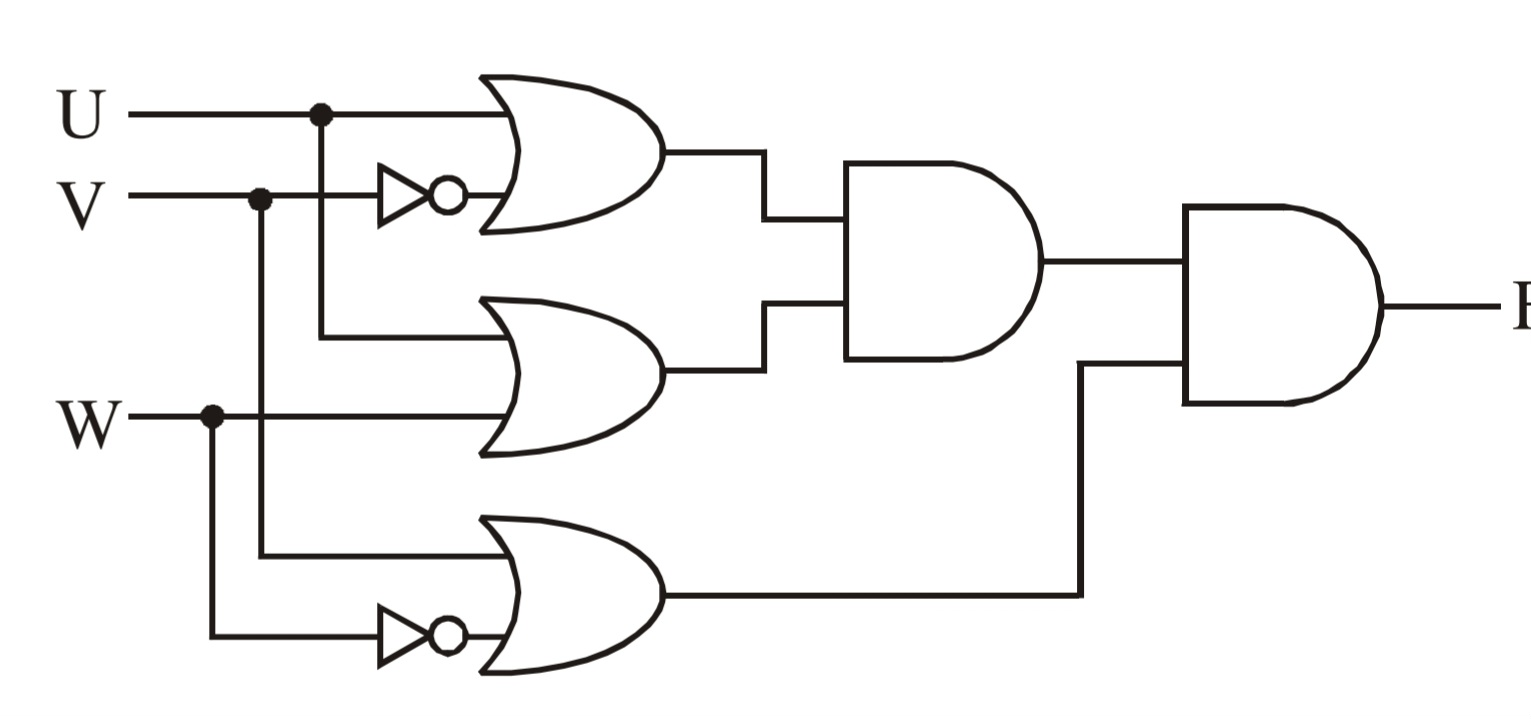
\includegraphics[width=\columnwidth]{figs/cbse-2016.jpg}
\caption{}
\label{fig:2016/c/6/b}
\end{figure}
\item Draw the logic circuit of the following Boolean Expression using only NAND Gates.
\hfill (CBSE 2017)
\label{prob:2017-1/c/6/b}
		\begin{align}
\label{eq:2017-1/c/6/b}
 XY + YZ
		\end{align}
\item Draw the Logic Circuit of the following Boolean Expression using only NOR Gates  
\hfill (CBSE 2017)
\label{prob:2017/c/6/b}
      \begin{align}
      (A+B)(C+D)
      \end{align}
\item Draw the Logic Circuit of the following Boolean Expression\hfill (CBSE 2018)
\begin{equation} 
(U'+V)(V'+W')
\end{equation}
\label{prob:2018/c/6/b}
\item Derive a Canonical POS expression for a Boolean function F, represented by 
Table \ref{tab:2019/c/6/c}\hfill (CBSE 2019)
\label{prob:2019/c/6/c}
\begin{table}[!ht]
\centering
\begin{tabular}{|l|l|l|c|}
	\hline
	X&Y&Z&F(X,Y,Z)\\
	\hline
	0&0&0&1\\
	0&0&1&0\\
	0&1&0&1\\
	0&1&1&0\\
	1&0&0&1\\
	1&0&1&1\\
	1&1&0&0\\
	1&1&1&0\\
	\hline
\end{tabular}
\caption{}
\label{tab:2019/c/6/c}
\end{table}
\item For the logic circuit shown in Fig.\ref{fig:2000/gate/ec/2/7}, find the simplified Boolean expression for the output. 
\label{prob:2000/gate/ec/2/7}
\hfill (GATE EC 2000)
\begin{figure}[!ht]
    \centering
    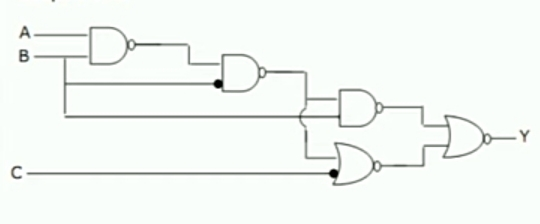
\includegraphics[width=\columnwidth]{figs/2000-gate-ec-2-7.jpg}
    \caption{}
\label{fig:2000/gate/ec/2/7}
\end{figure}
\item 
Obtain the Boolean Expression for the Logic circuit shown below
\label{prob:1993/gate/ec/4/8}
\hfill (GATE EC 1993)
	  	
	   \begin{circuitikz} \draw
(0,2) node[nand port] (mynand1) {}
(2,3) node[nand port] (mynand2) {}
(0,0) node[nand port] (mynand) {}
(2,-1) node[nand port] (mynand3) {}
(2,1) node[or port] (myor1) {}
(4,1) node[or port,number inputs =3] (myor2) {}
(mynand1.out) -- (myor1.in 1)
(mynand.out) -- (myor1.in 2)
(mynand2.out) -- (myor2.in 1)
(mynand3.out) -- (myor2.in 3)
(myor1.out) -- (myor2.in 2);
\node[left] at (mynand1.in 1) {\(A\)};
\node[left] at (mynand1.in 2) {\(B\)};
\node[left] at (mynand2.in 1) {\(A\)};
\node[left] at (mynand2.in 2) {\(A\)};
\node[left] at (mynand3.in 1) {\(C\)};
\node[left] at (mynand3.in 2) {\(C\)};
\node[left] at (mynand1.in 1)[ocirc] {};
\node[left] at (mynand.in 2) [ocirc] {};
\node[left] at (mynand.in 1) {\(B\)};
\node[left] at (mynand.in 2) {\(C\)};
\node[right] at (mynand1.out) {};
\node[right] at (mynand.out) {};
\node[right] at (mynand2.out) {};
\node[right] at (mynand3.out) {};
\node[right] at (myor2.out) {\(Y\)};
\end{circuitikz}
%
\item Implement Table
\ref{tab:1993/gate/ec/6/13}
using XNOR logic.
\label{prob:1993/gate/ec/6/13}
\hfill (GATE EC 1993)
\begin{table}[!ht]
	\centering
	\begin{tabular}{|c|c|c|}
		\hline
		\textbf{A}&\textbf{B}&\textbf{Y}\\
		\hline
		0&0&1\\
		\hline
		0&1&0\\
		\hline
		1&0&0\\
		\hline
		1&1&1\\   
		\hline 
	\end{tabular}
	\caption{}
\label{tab:1993/gate/ec/6/13}
\end{table}
\item 
\label{prob:1999-gate-ec-2-11}
For a binary half-sub-tractor having two inputs A and B, find the correct set of logical expressions for the outputs D (=A minus B) and X (=borrow).
\hfill (GATE EC 1999)
%
\item 
\label{prob:2007-gate-ec-43}
Find $X$ in the following circuit in Fig.
\ref{fig:2007-gate-ec-43}
\hfill (GATE EC 2007)
\begin{figure}[!ht]
\centering
	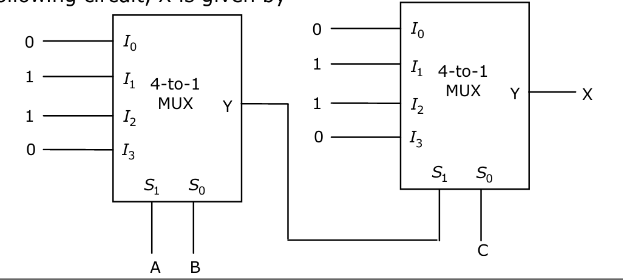
\includegraphics[width=1\columnwidth]{figs/2007-gate-ec-43.png}
\caption{}
\label{fig:2007-gate-ec-43}
\end{figure}
\item 
\label{prob:2007-gate-in-10}
      A logic circuit implements the boolean function F=X'.Y+X.Y'.Z'. It is found that the input combination X=Y=1 can never occur. Taking this into account, find a simplified expression for F. 
\hfill (GATE IN 2007)
\item 
\label{prob:2010-gate-ec-39}
Find the Boolean logic realised by the following circuit in Fig.
\ref{fig:2010-gate-ec-39}
\hfill (GATE EC 2010)
\begin{figure}[!ht]
\centering
	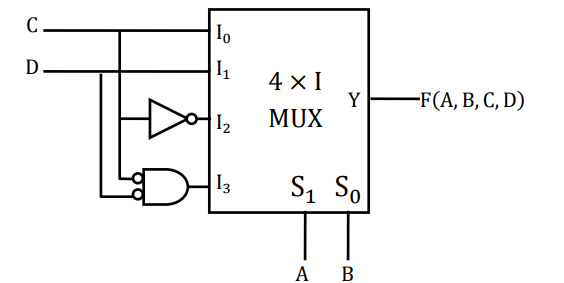
\includegraphics[width=1\columnwidth]{figs/2010-gate-ec-39.png}
\caption{}
\label{fig:2010-gate-ec-39}
\end{figure}
\item 
\label{prob:2011-gate-ec-20}
Find the logic function implemented by the circuit given below 
in Fig.
\ref{fig:2011-gate-ec-20}
\hfill (GATE EC 2011)
\begin{figure}[!ht]
\centering
	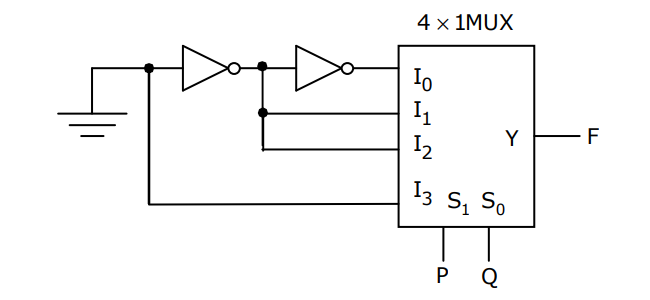
\includegraphics[width=\columnwidth]{figs/2011-gate-ec-20.png}
\caption{}
\label{fig:2011-gate-ec-20}
\end{figure}
\item
\label{prob:2016/gate/in/19}
Find F in the Digital Circuit given in the figure below
in Fig. \ref{fig:2016/gate/in/19}.
\hfill (GATE IN 2016)
\begin{figure}[!ht]
	\centering
\begin{tikzpicture}
 

 
% Logic ports
\node[nand port] (a) at (2,1){};
\node[nand port] (b) at (2,4){};
\node[nand port] (c) at (4,0){};
\node[nand port] (d) at (6,3){};

 
% Connection

 
\draw (a.in 2) -| (b.in 2);
\draw (b.out) -| (d.in 1);
 
\draw (a.out) -|  (c.in 1);
\draw (c.out) -| (d.in 2);
\draw (d.out) -- ++(1,0) node[near end,above]{F};
 
\draw (b.in 1) -- ++(-1.5,0)node[left](In1){X};
\draw (b.in 2) -- ++(-1.5,0)node[left](In3){Y};
\draw (c.in 2) -- ++(-1.5,0)node[left](In3){Z};
% Jump crossing element
1
\end{tikzpicture}
	\caption{}
\label{fig:2016/gate/in/19}
\end{figure}


\item 
\label{prob:2017-gate-ec-16}
Find the logic function implemented by the circuit given below 
in Fig.
\ref{fig:2017-gate-ec-16}
\hfill (GATE EC 2017)
\begin{figure}[!ht]
\centering
	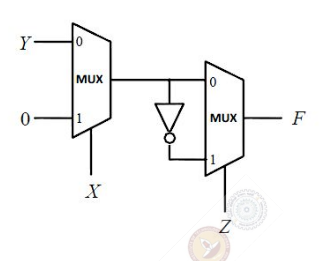
\includegraphics[width=\columnwidth]{figs/2017-gate-ec-16.png}
\caption{}
\label{fig:2017-gate-ec-16}
\end{figure}
\item 
\label{prob:2018-gate-ec-31}
Find the logic function implemented by the circuit given below 
in Fig.
\ref{fig:2018-gate-ec-31}
\hfill (GATE EC 2018)
\begin{figure}[!ht]
\centering
	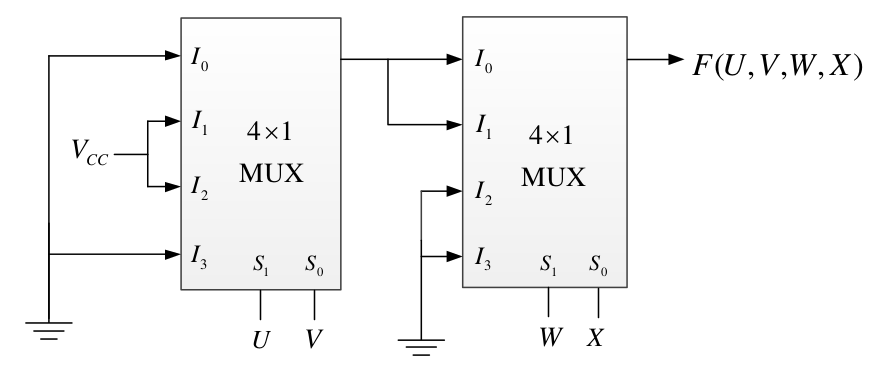
\includegraphics[width=\columnwidth]{figs/2018-gate-ec-31.png}
\caption{}
\label{fig:2018-gate-ec-31}
\end{figure}
\item 
\label{prob:2018-gate-ee-14}
Find the logic function implemented by the circuit given below 
in Fig.
\ref{fig:2018-gate-ee-14}
\hfill (GATE EE 2018)
\begin{figure}[!ht]
\centering
	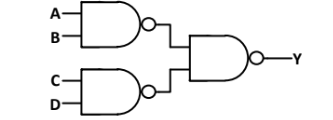
\includegraphics[width=\columnwidth]{figs/2018-gate-ee-14.png}
\caption{}
\label{fig:2018-gate-ee-14}
\end{figure}
\item 
\label{prob:2019-gate-ee-36}
Find the logic function implemented by the circuit given below 
in Fig.
\ref{fig:2019-gate-ee-36}
\hfill (GATE EE 2019)
\begin{figure}[!ht]
\centering
	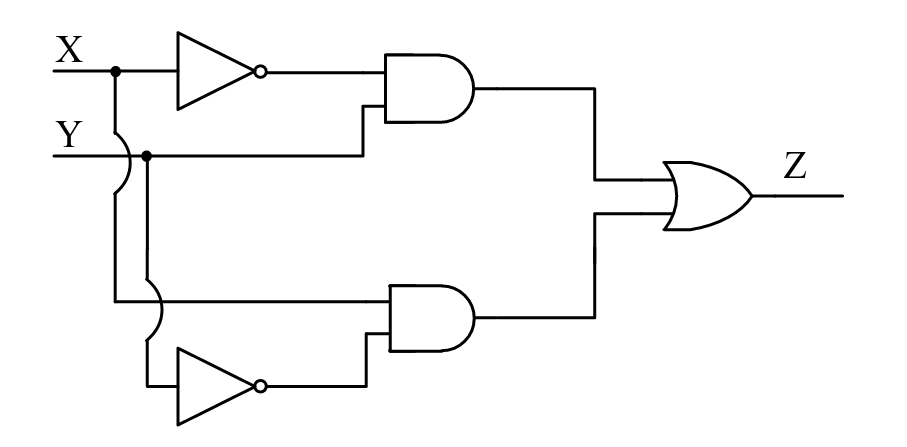
\includegraphics[width=\columnwidth]{figs/2019-gate-ee-36.png}
\caption{}
\label{fig:2019-gate-ee-36}
\end{figure}
\item 
\label{prob:2018-gate-CS-4}		
Let $\oplus$ and $\odot$ denote the Exclusive OR and Exclusive NOR operations, respectively.Which one of the following is NOT CORRECT
\ref{fig:2018-gate-CS-4}
\hfill (GATE CS 2018)
\begin{enumerate}[label=(\Alph*)]
    \item $\overline{P\oplus Q}$ = $ P \odot Q $
    \item $\overline{P} \oplus Q$ = $ P \odot Q $
    \item $\overline{P} \oplus \overline{Q}$ = $ P \oplus Q $
    \item $(P \oplus \overline{P}) \oplus Q$ = $(P \odot \overline{P}) \odot \overline{Q}$
\end{enumerate}
\end{enumerate}
